\section{Koordinatensysteme und Koordinatentransformationen}

\begin{figure}[htb] % [htb]
  \centering
  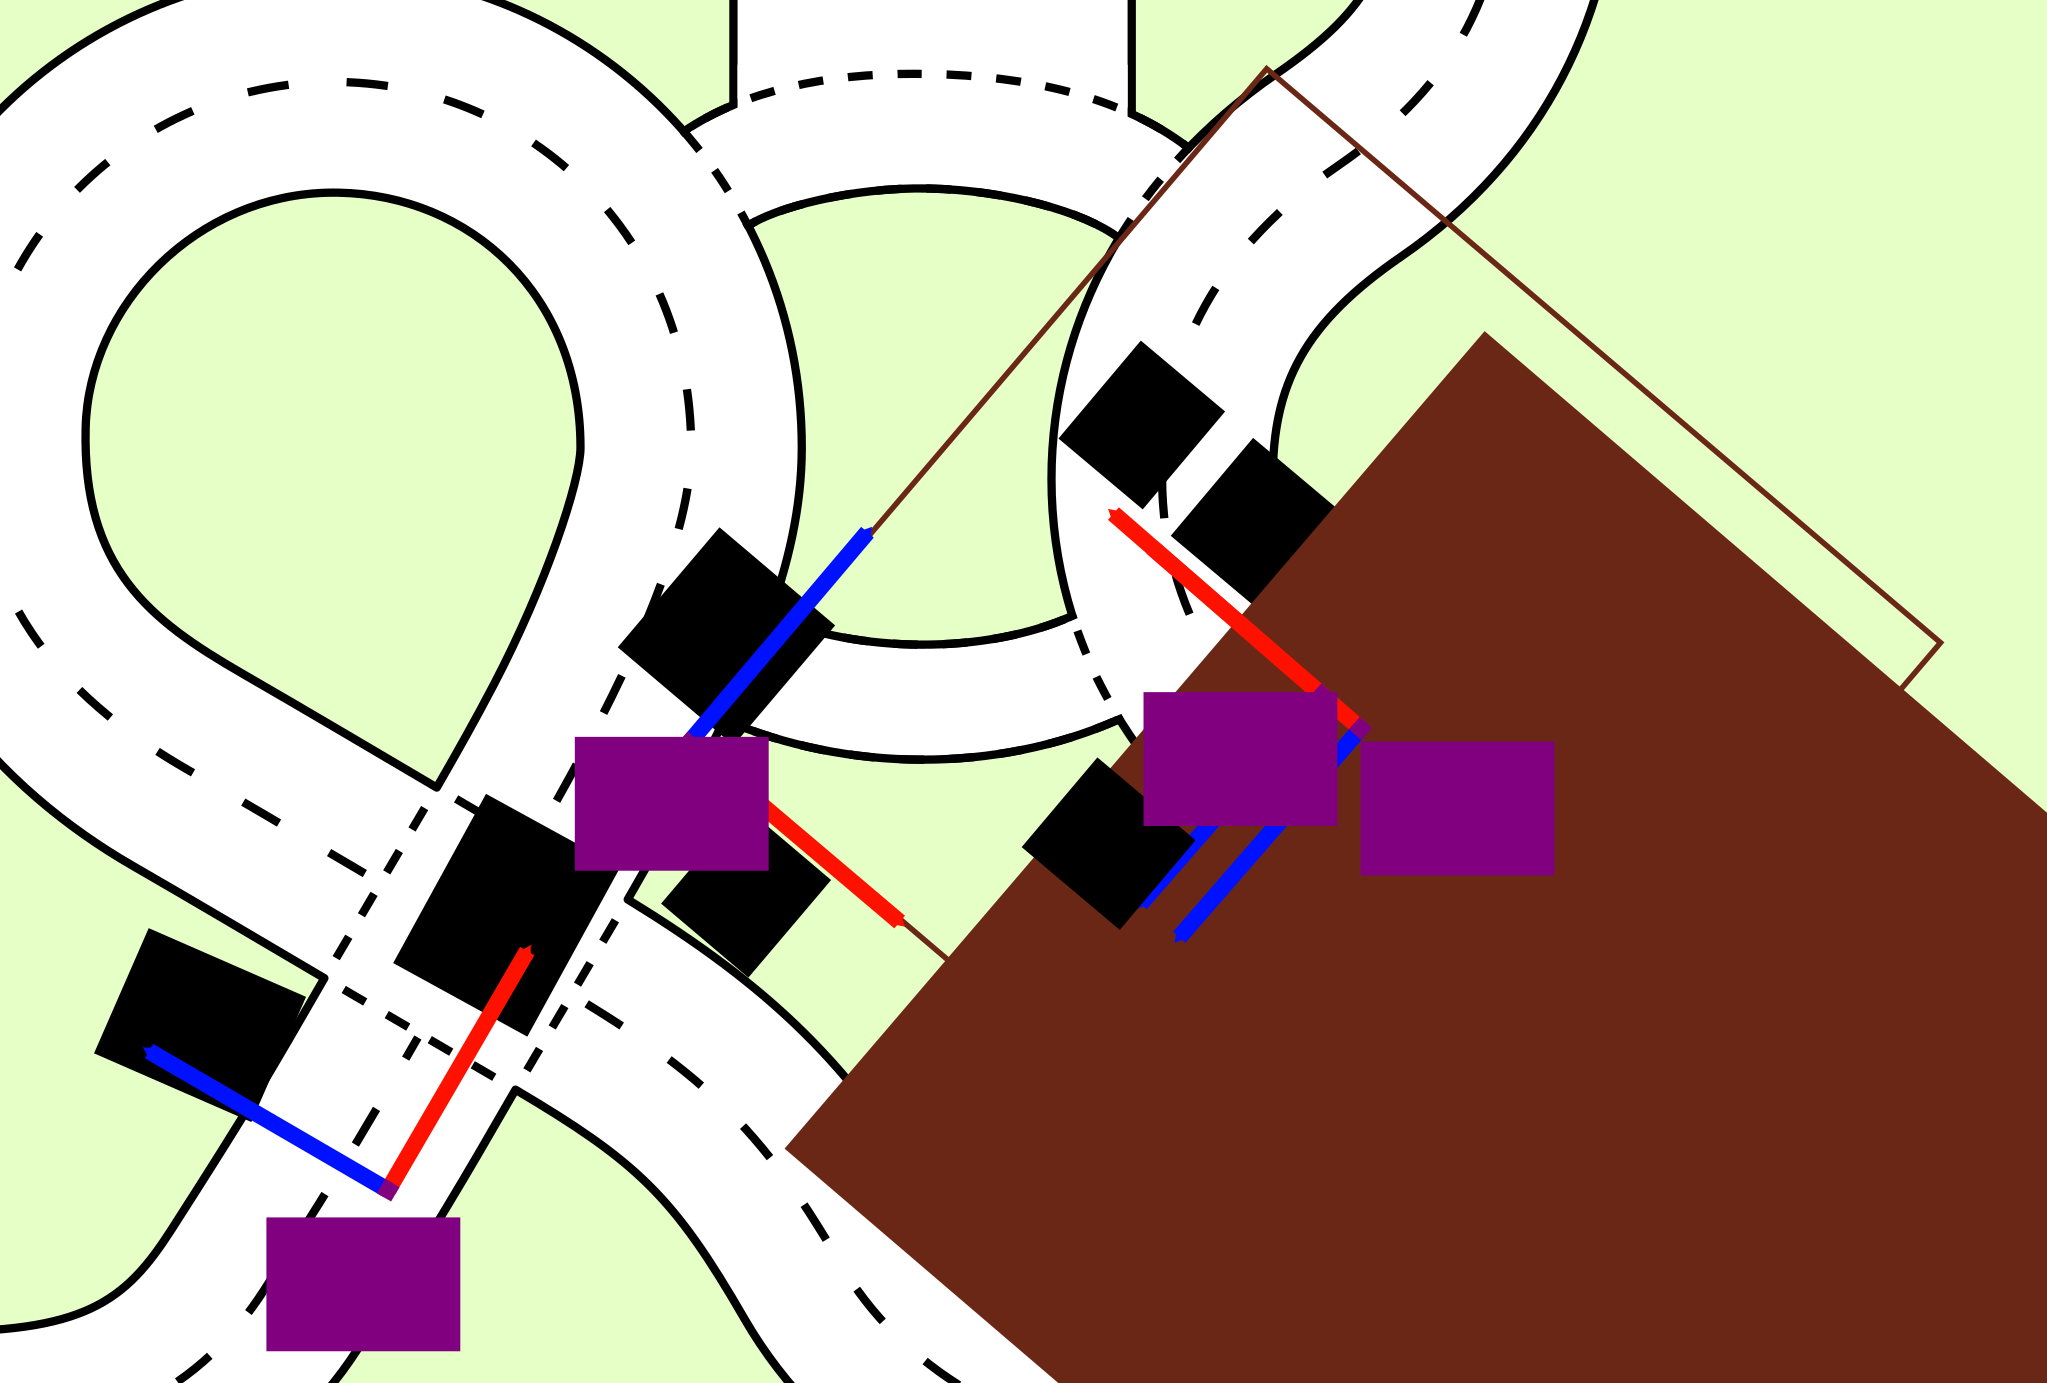
\includegraphics[width=0.9\textwidth]{grundlagen_kos.pdf}
  \caption{Alle eingeführten Koordinatensysteme im Überblick}
  \label{fig:grundlagen_kos}
\end{figure}

Um ein Modellauto steuern zu können, werden unter anderem die Informationen über den aktuellen Standort und den Zielpunkt, den das Fahrzeug ansteuern soll, benötigt. Die Trajektorie ist wiederum davon abhängig, an welcher Stelle sich die Fahrbahnmarkierungen befinden. Alle Positionen von Objekten im Raum werden deshalb mit Entfernungen relativ zu entsprechenden Koordinatensystemen beschrieben. Für die Beschreibung unseres TUCar auf dem Parcour und die Lage der Straßenlinien eignet sich das kartesische Koordinatensystem besser als Polar- oder Kugelkoordinaten. Letztendlich wurden drei Koordinatensysteme festgelegt, welche in Abbildung ~\ref{fig:grundlagen_kos} verdeutlicht werden. 

Das Weltkoordinatensystem bildet die Basis und ist an einem beliebigen Punkt des Szenarios festgemacht. Es dient zur Beschreibung der Pose des mobilen Roboters und der Linienpunkte in der Weltkarte. Damit sich die Pixelkoordinaten nicht von der Matrixindizierung unterscheiden, wird das Bildkoordinatensystem in die linke obere Ecke des entzerrten Fotos gelegt. So zeigt die x-Achse in Richtung der Zeilen und die Spalten sind gleich der y-Koordinate. In der Hinterachse des Autos liegt das Roboterkoordinatensystem, welches in der Lage zum Weltkoordinatensystem die Pose darstellt.

Um einen Punktvektor von einem in ein anderes Koordinatensystem zu transformieren, bedarf es einer Verschiebung (Translation) in Richtung eines Verschiebungsvektors und einer Drehung (Rotation) um eine Achse. Da sich unser Roboter nur in der xy-Ebene bewegt, wird hier also nur um die z-Achse gedreht.  

% Formel für R = Rot(z,\theta) //(Rotationsmatrix)
\begin{equation}
\mathbf{R} = Rot(z,\theta) = 
\begin{pmatrix}
\cos{\theta} & -\sin{\theta} & {0} 	\\
\sin{\theta} & \cos{\theta} & {0} 	\\
{0} & {0} & {1} 				    	\\
\end{pmatrix}
\end{equation}

Und weiter im Text ...
